\documentclass{article}
% General document formatting
\usepackage[margin=0.7in]{geometry}
\usepackage[parfill]{parskip}
\usepackage[utf8]{inputenc}
% Related to math
\usepackage{amsmath,amssymb,amsfonts,amsthm}

% sumniki
\usepackage[slovene]{babel}

% fix bordermatrix
\usepackage{etoolbox}
\let\bbordermatrix\bordermatrix
\patchcmd{\bbordermatrix}{8.75}{4.75}{}{}
\patchcmd{\bbordermatrix}{\left(}{\left[}{}{}
\patchcmd{\bbordermatrix}{\right)}{\right]}{}{}

% images
\usepackage{graphicx}
\graphicspath{ {./images/} }

% theorems
\theoremstyle{definition}
\newtheorem{definition}{Definicija}[section]
\newtheorem{lemma}{Lema}[section]
\newtheorem{conseq}{Posledica}[section]
\newtheorem{claim}{Trditev}[section]
\newtheorem{theorem}{Izrek}[section]

% I like my squares DARK
\renewcommand\qedsymbol{$\blacksquare$}

\begin{document}
	\selectlanguage{slovene} % sumniki
	
	\title{Teorija grafov - zapiski predavanj prof. Klav"zarja}
	\author{Yon Ploj}
	\date{2. semester 2021}
	\maketitle
	
	
	% 16. 02. 2021
	\section{Osnovni pojmi}
	$ G = (V(G), E(G)) $ \\ 
	$ V(G) = \left\lbrace u, v, w, x, y, z\right\rbrace $ \\ 
	$ E(G) = \left\lbrace\left\lbrace u,v\right\rbrace, \left\lbrace u,x\right\rbrace, \left\lbrace u,y\right\rbrace, \left\lbrace w,x\right\rbrace, \left\lbrace w,y\right\rbrace, \left\lbrace y,z\right\rbrace\right\rbrace $ (neurejeni pari) \\ 
	Definiramo: vozli"s"ce, povezava, sosednja vozli"s"ca, inciden"cni povezavi
	
	Skica grafa:
	\begin{itemize}
		\item vozli"s"cem injektivno priredimo to"cke v ravnini.
		\item povezave ponazorimo s krivuljo med kraji"s"cema povezave.
	\end{itemize}
	
	\begin{definition}[Sose"s"cina vozli"s"ca]
		$N_g(v) := \left\lbrace u \in V(G): uv \in E(G)\right\rbrace$ % <- N as in neighbourhood
	\end{definition}
	\begin{definition}[Stopnja vozli"s"ca]
		$deg(v) := |N_g(v)|$
		$$\delta(G) := \underset{v \in V(G)}{min} \lbrace deg(v) \rbrace $$
		$$\Delta(G) := \underset{v \in V(G)}{max} \lbrace deg(v) \rbrace $$		
		% delta je minimalna stopnja vozlisca v $G$
		% Delta je maksimalna stopnja vozlisca v $G$
	\end{definition}
	\begin{definition}[Izolirano vozli"s"ce]
		$deg(v) = 0$
	\end{definition}
	\begin{definition}[List grafa]
		$deg(v) = 1$
	\end{definition}
	\begin{definition} [k-regularen graf]
		Graf, kjer je vsako vozli"s"ce stopnje $k$
	\end{definition}
	\begin{definition} [Kubi"cni graf]
		3-regularen graf
	\end{definition}	
	
	\begin{definition}[Matrika sosednosti]
	$A_{ij} = \begin{cases}1; v[i] \sim v[j] \\ 0; \text{sicer} \end{cases}$
	$$
		A(G) =
		\bbordermatrix{
			    & v_1 & v_2 & v_3 & v_4 &\ldots& v_n \cr
			v_1 &  0  &  1  &  0  &  1  &      &  0  \cr
			v_2 &  1  &  0  &  1  &  0  &      &  0  \cr
			v_3 &  0  &  1  &  0  &  0  &      &  0  \cr
			v_4 &  1  &  0  &  0  &  0  &      &  0  \cr
		 \vdots &     &     &     &     &\ddots&     \cr
			v_n &  0  &  0  &  0  &  0  &      &  0  \cr
		}
	$$
	\end{definition}
	je vedno simetri"cna po diagonali (ker $u \sim v \iff v \sim u$)
	diagonala so ni"cle (ker $\forall v: \lnot(v \sim v)$)
	
	
	\begin{definition}[Inciden"cna matrika] 
		$B_{ij} = \begin{cases}1; v[i] \in e[j] \\ 0; \text{sicer} \end{cases}$
		
		$$
			B(G) =
			\bbordermatrix{
			    & e_1 & e_2 & e_3 & e_4 &\ldots& e_6 \cr 
			v_1 &  1  &  1  &  0  &  0  &      &  0 \cr 
			v_2 &  0  &  0  &  0  &  1  &      &  1 \cr
		 \vdots &     &     &     &     &\ddots&    \cr
			v_n &  0  &  1  &  1  &  1  &      &  0 \cr
			}
		$$
		vsak stolpec ima natanko 2 enici (vsaka povezava ima natako 2 kraji"s"ci)
	\end{definition}
	
	\begin{lemma}[Lema o rokovanju]
		za vsak G velja
		\[ \sum_{v \in V(G)} (deg(v)) = 2*|E(G)| \]
		\begin{proof}
			"Stevilo enic v inciden"cni matriki je "stevilo stolpcev $*$ 2 (ker ima vsak stolpec natanko 2 enici). "Stevilo stolpcev je $|E(G)|$.
			V vrstici $v_i$ je $deg(v_i)$ enic. "Ce se"stejemo "stevilo enic po vrsticah = "stevilo enic po stolpcih = $\sum_{v \in V(G)}(deg(v)) = 2*|E(G)|$
		\end{proof}
	\end{lemma}
	
	\begin{conseq} 
		V poljubnem grafu je "stevilo vozli"s"c lihe stopnje sodo mnogo. 
		\begin{proof}
			\[ 2*|E(G)| = \sum_{v}(deg(v)) = \sum_{v \text{ sodo}}(deg(v)) + \sum_{v \text{ liho}}(deg(v)) \] 
			Prvi "clen je sodo "stevilo in vsota je sodo "stevilo. Torej je drugi "clen sodo "stevilo. Torej je sumandov v drugi vsoti sodo mnogo.
		\end{proof}
	\end{conseq}
	
	\begin{claim} 
		Ne obstaja kubi"cen graf na 9 vozli"s"cih
	\end{claim}
	
	
	\subsection{Podgrafi}
	\begin{definition}[Podgraf]
		Graf H je podgraf G, "ce je $V(H) \subseteq V(G)$ in $E(H) \subseteq E(G)$. Pi"semo $H \leq G$
	\end{definition}
	\begin{definition}[Vpeti podgraf]
		$V(H) = V(G) \land E(H) \subseteq E(G)$
	\end{definition}
	\begin{definition}[Inducirani graf]
		Vsak $v_1v_2 \in E(H)$: ($\left\lbrace v_1,v_2\right\rbrace \subseteq V(H) \implies \left\lbrace v_1,v_2\right\rbrace \subseteq V(G)$)
		\\
		Podgraf dobimo, "ce zbri"semo nekaj vozli"s"c in pripadajo"cih robov, ne pa drugih robov.
		Inducirani podgraf je natan"cno dolo"cen z mno"zico vozli"s"c (katera smo odstranili).
	\end{definition}
	
	\subsection{Dru"zine grafov} 
	\begin{definition}[Polni graf]
		$K_n$; $|V| = n$, vsak par vozli"s"c je soseden.
	\end{definition}

	$K_3$ = trikotnik.
	
	$|E(K_n)| = \frac{n(n-1)}{2} = {n \choose 2}$ (dokaz z lemo o rokovanju)
	
	\begin{definition}[Pot na n vozli"s"cih]
		$P_n$;
		\\
		$V(P_n) = \left\lbrace v_1, v_2, \ldots ,v_n \right\rbrace$; 
		\\
		$E(P_n) = \left\lbrace\left\lbrace v_i, v_{i+1} \right\rbrace : i \in [n-1]\right\rbrace = \left\lbrace \left\lbrace i, i+1 \right\rbrace; i \in Z_n \backslash \left\lbrace n-1\right\rbrace\right\rbrace$ \\ 
	\end{definition}
	\begin{definition}[Cikel na n vozli"s"cih]
		$C_n = (V(C_n), E(C_n))$ \\
		$V(C_n) = Z_n$ \\
		$E(C_n) = \left\lbrace\left\lbrace i,i+1\right\rbrace; i \in Z_n\right\rbrace$
	\end{definition}

	Limitacije:
	\begin{itemize}
		\item $K_n: n \geq 0$ 
		\item $P_n: n \geq 0$ 
		\item $C_n: n \geq 3$
	\end{itemize}

	"Ce v $C_n$ zbri"semo poljubno povezavo, dobimo vpeti $P_n$.
	
	\subsection{Polni dvodelni grafi}
	\begin{definition}[Poln dvodelni graf]
		$K_{m,n}$; $m,n \geq 0$ \\ 
		je graf, za katerega obstajata mno"zici A in B, tako da je
		$$ \forall u \in A, v \in B: \left\lbrace u,v \right\rbrace \in E(K_{m,n})$$
		oziroma
		$$E(K_{m,n}) = \left\lbrace\left\lbrace u,v\right\rbrace: u \in A, v \in B\right\rbrace$$
		$|A| = m, |B| = n$ 		
	\end{definition} 
	\begin{definition}[Zvezde]
			Grafi oblike $K_{1,n}$
	\end{definition}
	$K_{2,2} = C_4$
	
	\begin{definition}[d-kocka $Q_d$]
		Graf oblike $V(Q_d) = \left\lbrace 0,1 \right\rbrace ^n$ \\
		(potenca ozna"cuje kartezi"cni produkt) \\
		$= \left\lbrace (b_1, \ldots, b_n): b_i \in \left\lbrace 0,1\right\rbrace\right\rbrace \text{ (binarni niz dol"zine n) }$
	\end{definition}

	Limitacije:
	\begin{itemize}
		\item $d \geq 1$
	\end{itemize}
	
	Vozli"s"ci $\left\lbrace b_1, b_2, b_3, \ldots \right\rbrace$ in $\left\lbrace b_1', b_2', b_3', \ldots \right\rbrace$ sta sosednji $\iff$ obstaja natanko en $i \in [n]: (b_i \neq b_i')$
	
	$Q_n$ je $n$-regularen graf; $deg(b_1) = deg(b_2) = \ldots = n$.
	

	\subsection{Posplo"seni Petersenovi grafi $P_{n,k}$} 
	\begin{definition}[Petersenov graf]
		$$V(P_{n,k}) = \left\lbrace u_0, \ldots, u_{n-1} \right\rbrace \dot\cup \left\lbrace v_0, \ldots, v_{n-1} \right\rbrace $$  % \dot\cup = diskunktivna unija
		$$E(P_{n,k}) = \left\lbrace\left\lbrace u_i,u_{i+1}\right\rbrace: i \in Z_n\right\rbrace \dot\cup \left\lbrace \left\lbrace u_i,v_i \right\rbrace: i \in Z_n \right\rbrace \dot\cup \left\lbrace\left\lbrace v_i,v_{i+n} \right\rbrace: i \in Z_n\right\rbrace$$ 
		U-ji so povezani v cikel. Enakole"zni Uji in Vji so povezani. Vji so povezani s preskoki po k.
		\\
		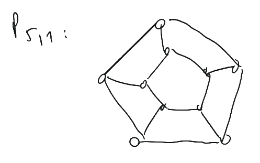
\includegraphics{petersenovi51}
		% no line break here, to keep both images side by side
		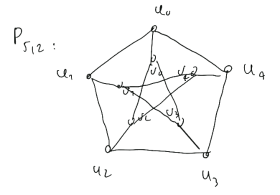
\includegraphics{petersenovi52}
		\\
		Petersenov graf je nek bad boy ker pokvari veliko izrekov.
	\end{definition}

	Limitacije:
	\begin{itemize}
		\item $n \geq 3$
		\item $2k < n$ 
	\end{itemize}

	
	
	\begin{definition}[Kro"zni grafi] 
		$S \subseteq Z_n; 0 \notin S \land s \in S \implies (n-s) \in S$
	\end{definition}
	$Cir(n, S)$: vozli"s"ca tvori $Z_n$, povezave: $\left\lbrace uv, v-u \in S\right\rbrace$ \\ 
	$K_n = Cir(n, [n-1])$ \\ 
	$C_n = Cir(n, \left\lbrace1, n-1\right\rbrace)$
	
	\begin{definition}[Enostaven graf]
		Graf je enostaven, "ce nima ve"ckratnih povezav ali zank. Za nas je graf $\iff$ enostaven graf.
	\end{definition}
	\begin{definition}[Digrafi]
		Usmerjeni grafi (mi ne poznamo)
	\end{definition}
	\begin{definition}[Obte"zeni grafi]
		mi "se ne poznamo
	\end{definition}
	
\section{Poti, cikli in dvodelnost}
	% 23. 02. 2021
	\begin{definition}[Sprehod]
		Zaporedje vozli"s"c $v_0,v_1,v_2,\ldots,v_k$, da je $v_i \sim v_{i+1}$ za $i \in \left\lbrace 0, \ldots, k-1 \right\rbrace $ 
	\end{definition}
	\begin{definition}[Enostaven sprehod]
		Povezave se ne ponavljajo (vozli"s"ca pa lahko)
	\end{definition}
	\begin{definition}[Sklenjen sprehod]
		$v_0 = v_k$
	\end{definition}
	\begin{definition}[Pot v grafu]
		(Enostaven) sprehod, kjer so vsa vozli"s"ca razli"cna (torej tudi povezave razli"cne)
	\end{definition}
	\begin{definition}[Dol"zina sprehoda]
		"St. povezav v sprehodu
	\end{definition}
	\begin{definition}[Cikel v grafu]
		Sklenjen sprehod, v katerem so vsa vozli"s"ca razli"cna
	\end{definition}

	\begin{lemma}
		"Ce med dvema vozli"s"cema obstaja sprehod dolzine $k$, potem med njima obstja tudi pot dol"zine kve"cjemu $k$.
		\begin{proof}
			Naj bosta $u,v \in V(G)$ in $u=x0,x1,...,xk=v$ je uv-sprehod. "Ce so vsa vozli"s"ca paroma razli"cna, je to iskana pot. Sicer se nek x ponovi. Naj bo $x_i$ prvo tako vozli"s"ce, $x_j$ pa druga pojavitev $x_i$. Sprehod $x_0, \ldots, x_i, x_{j+1}, \ldots, x_k$ je kraj"si od originalnega, in ima manj ponovitev. "Ce je ta sprehod pot, je to iskana pot. Sicer ponavljamo postopek dokler ne najdemo iskane poti.
		\end{proof}
	\end{lemma}
	
	\begin{lemma}
		"Ce med vozli"s"cem grafu $u$ in $v$ obstajata dve razli"cni poti, potem $G$ vsebuje vsaj en cikel.
		\begin{proof}
			Naj bosta $P$ in $Q$ $u,v$-poti v $G$. "Ce je $V(P) \cap V(Q) = \left\lbrace u,v\right\rbrace$, potem je $P$ unija $Q$ iskani cikel. Sicer poi"s"cemo prvo vozli"s"ce $x$ na $Q$, da ni na $P$ (obstaja ker $P \neq Q$). Nato poi"s"cemo prvo naslednje vozli"s"ce $y$ na $Q$, da je tudi na $P$ (obstaja, ker se $P$ in $Q$ sre"cata vsaj na $v$). Tedaj podpot od $P$ med $x$ in $y$ ter podpot od $Q$ med $x$ in $y$ tvorita iskani cikel na $G$.
		\end{proof}
	\end{lemma}
	
	\begin{lemma}\label{lem:1}
		"Ce ima graf sklenjen sprehod lihe dol"zine, potem vsebuje tudi cikel lihe dol"zine.
		\begin{proof}
			(indukcija po dol"zini sprehoda k)\\
			BI: $k=3$ OK \\ 
			IK: $n-1 \implies n$ \\ 
			Naj bo $S=v_0,v_1,\ldots,v_n=v_0$ sprehod lihe dol"zine. "Ce so vsa vozli"s"ca razli"cna, imamo lih cikel. Sicer obstaja $i$,$j$ da $(0 \leq i < j) \land (v_i = v_j)$. Vsota dol"zin sprehodov $v_0, \ldots, v_i, v_{j+1}, \ldots, v_n = v_0$ in $v_j = v_i, v_{i+1},\ldots,v_{j-1},v_j=v_i$ je liha. Torej je natanko eden od teh sprehodov lih. Oba sprehoda sta strogo kraj"sa od originalnega sprehoda. IP zagotavlja, da ima lih od sprehodov lih cikel.
		\end{proof}
	\end{lemma}

	
	Definirajmo relacijo $R$: $xRy \iff$ med $x$ in $y$ obstaja pot.
	\begin{claim}
		$R$ je ekvivalen"cna
	\end{claim}
	Ekvivalen"cnim razredom $R$ pravimo komponente grafa \\ 
	$\Omega(G) =$ "stevilo komponent \\ 
	\begin{definition}[Povezan graf]
		$\Omega(G) = 1$
	\end{definition}
	\begin{definition}[Razdalja $d_G(u,v)$]
		je "stevilo povezav na najkraj"si $uv$ poti v $G$. "Ce taka pot ne obstaja, je $d(u,v) = \infty$
	\end{definition}
	
	\begin{claim}
		$(V(G), d_G)$ je metri"cni prostor. \\
			$\implies (d_G(u,v) \geq 0) \land (d_G(u,v) = 0 \iff u = v)$ \\ 
			$\implies d_G(u,v) = d_G(v,u)$ \\ 
			$\implies d_G(u,v) \leq d_G(u,w) + d_G$
	\end{claim}
	
	\begin{definition}[Ekscentri"cnost]
		$ecc_g(u) = max_{x \in V(G)}\left\lbrace d_G(u,x)\right\rbrace$
	\end{definition}
	\begin{definition}[Premer $diam(G)$]
		je najve"cja ekscentri"cnost
	\end{definition}
	\begin{definition}[Polmer $rad(G)$]
		je najkraj"sa ekscentri"cnost
	\end{definition}
	\begin{definition}[O"zina ali notranji premer]
		je dol"zina najkraj"sega cikla. "Ce graf nima cikla, je o"zina $= \infty$.
	\end{definition} 
	
	\begin{definition}[Dvodelnost] 
		$G$ je dvodelen, "ce lahko $V(G)$ razdelimo v disjunktni mno"zici $A$ in $B$, da $uv \in E(G) => u \in A \land v \in B$ ali obratno. \\ 
		Pravimo, da sta $A$ in $B$ neodvisni. (Ni povezave znotraj mno"zice)
	\end{definition}
	
	\begin{claim} 
		Vse kocke so dvodelne.
		\begin{proof}
			z indukcijo (dvodelno pove"zemo dve $n-1$ kocki)
		\end{proof} 
	\end{claim}
	
	\begin{theorem}
		Graf $G$ je dvodelen natanko tedaj ko ne vsebuje lihih ciklov. 
		\begin{proof} 
			($\Rightarrow$) lihi cikli niso dvodelni, zato tudi graf z lihim ciklom ne more biti dvodelen. \\ 
			($\Leftarrow$) predpostavimo lahko, da je $G$ povezan. ("Ce ni povezan, je dvodelen natanko tedaj, ko so vse komponente dvodelne). Vzemimo vozli"s"ce $v_0$. Definirajmo $A=\left\lbrace x \in V(G): d(v_0, x) \text{ je sodo}\right\rbrace$ in $B=\left\lbrace x \in V(G): d(v0, x) \text{ je liho}\right\rbrace$ (tukaj nam pomaga, da smo predpostavili povezanost, saj nam neskon"cnost ne dela preglavic). O"citno je $A \cap B = \left\lbrace/\right\rbrace$. $A \cup B = V(G)$. Poka"zimo, da je $(A,B)$ dvodelna razdelitev (znotraj $A$ in znotraj $B$ ni povezav): naj bosta $u,w \in A$. Lo"cimo 3 primere:
			\begin{enumerate}
				\item $|d(v_0, u) - d(v_0, w)| \geq 2$ \\
				Tedaj $uw \not\in E(G)$. To je res, sicer bi dobili:
				$$\text{B"SS } d(v_0, u) < d(v_0, w)$$
				"Ce bi obstajala $uw$, potem je
				$$d(v_0,w) \leq d(v_0, u) + d(u,w) = d(v_0, u) + 1$$
				To je bodisi o"citno, lahko pa temu re"cete tudi trikotni"ska neenakost.
				
				\item $|d(v_0, u) - d(v_0, w)| = 1$ \\
				Vemo, da to ni mo"zno, ker sta obe iz mno"zice $A$, torej sta obe razdalji sodi, desna stran pa liha.
				
				\item $d(v_0, u) = d(v_0, w) = k$ \\
				Recimo, da obstaja povezava $uw$. Naj bo $P$ poljubna najkraj"sa $v_0,u$-pot in $Q$ poljubna najkraj"sa $v_0,w$-pot. Poglejmo $P \cup Q \cup \lbrace u w \rbrace$. $P$ in $Q$ nista nujno notranje disjunktni, toda $P \cup U \cup \lbrace u w \rbrace$ je sklenjen sprehod
				($v_0 \overset{P}{\rightarrow} u,w \overset{Q}{\rightarrow} v_0 $) z dol"zino $|P| + 1 + |Q| = 2k+1$.
				Po lemi \ref{lem:1} vemo, da imamo v $G$ nek lih cikel. To je v nasprotju s predpostavko. 
			\end{enumerate}
			Dokazali smo, da je mno"zica $A$ neodvisna. Dokaz za mno"zico $B$ poteka na enak na"cin.
		\end{proof}
	\end{theorem}
	Ko se bomo pogovarjali o barvanju grafov, bomo karakterizirali dvodelne grafe tudi s kromati"cnim "stevilom.
	
	\section{Morfizmi grafov}
	% 02. 03. 2021
	
	\begin{definition}[Homomorfizem]
		Preslikava $f: V(G) \rightarrow V(H)$ je homomorfizem ntk. $u \sim v \Rightarrow f(u) \sim f(v)$
	\end{definition}
	\begin{definition}[Epimorfizem]
		Surjektiven homomorfizem 
	\end{definition}
	\begin{definition}[Monomorfizem (vlo"zitev)]
		Injektiven homomorfizem ($G$ je podgraf v $H$) 
	\end{definition}
	\begin{definition}[Izometri"cna vlo"zitev]
		"Ce je $d(x,y) = d(f(x), f(y))$ za vsak $x$,$y$
	\end{definition}
	\begin{definition}[Avtomorfizem]
		Izomorfna preslikava $G \rightarrow G$
	\end{definition}
	\begin{definition}[Asimetri"cen graf]
		Graf katerega edini avtomorfizem je $id$
	\end{definition}
	
	
	\section{Operacije z grafi in k-povezanost}	
	\begin{definition}[Komplement $G$]
		$\overline{G} := (V(G), \overline{E(G)})$
	\end{definition}
	%\begin{definition}[Avtomorfizem]
	$P_4$ je sebi-komplementaren
	
	Grupa avtomorfizmov $G$ in $\overline{G}$ je enaka.
	
	"Ce $G$ ni povezan, je $diam(\overline{G}) \leq 2$
	
	\begin{definition}[Skr"citev]
		Odstranimo povezavo in identificiramo vozli"s"ci ki jih povezuje.
		Morebitne podvojene povezave odstranimo.
	\end{definition} 
	
	% 09. 03. 2021
	\begin{definition}[Minor]
		$H$ je minor grafa $G$, "ce $G$ premore podgraf $X$ in mno"zico povezav $F \subseteq E(X)$, tako da je $H$ dobljen s skr"citvijo povezav iz $F$.
		Ozna"cimo $H = X \backslash F$ (V tem primeru $ \backslash $ pomeni skr"citev povezav)
	\end{definition} 
	
	\begin{claim}
		Vrstni red skr"citev ni va"zen
	\end{claim}
	
	\subsection{Subdividiranje} 
	"Ce povezavo nadomestimo s potjo dol"zine 2, smo povezavo subdividirali. Oznaka: $G^+(E)$ \\ 
	
	\begin{definition}[Subdividiranje]
		Neformalno: nekaj povezav nadomestimo s potmi. \\
		Formalno: naj bo $e = uv \in E(G)$
		$$ V(G^+(e)) = V(G) \cup \left\lbrace v_0\right\rbrace, v_0 \notin V(G) $$
		$$ E(G^+(e)) = (E(G)\left\lbrace uv\right\rbrace) \cup \left\lbrace u \sim v_0, v \sim v_0 \right\rbrace $$
	\end{definition}
	
	Graf $H$ je subdivizacija $G$, "ce $H$ dobimo iz $G$ prek zaporednega subdividiranja povezav.
	
	\begin{definition}[Glajenje vozli"s"c] Neformalno: obratna operacija subdividiranja. \\
		Formalno: 
		$$ V(G-(w)) = V(G) \backslash \left\lbrace w\right\rbrace $$ 
		$$ E(G-(w)) = (E(G) \backslash \left\lbrace uw, vw \right\rbrace) \cup \left\lbrace uv \right\rbrace $$
	\end{definition}
	
	\begin{definition}[Homeomorfizem]
		Grafa $G$ in $H$ sta homeomorfna, "ce postaneta izomorfna, ko zgladimo vsa vozli"s"ca stopnje 2 v obeh grafih.
	\end{definition}
	
	\begin{definition}[Kartezi"cni produkt grafov]
		$$ V(G \mathrel{\square} H) = V(G) \times V(H) $$
		$$ E(G \mathrel{\square} H) = \left\lbrace (g, k)(g', k'): (gg' \in E(G) \land k=k') \lor (g=g' \land kk' \in E(H)) \right\rbrace $$
	\end{definition}
	Lastnosti: (monoid)
	\begin{itemize}
		\item simetri"cnost
		\item asociativnost
		\item enota
	\end{itemize}

	$Q_n = (K_2)^n$
	
	\begin{definition}[Prerezno vosli"s"ce]
		$v$ je prerezno, "ce ima $G-v$ ve"c komponent kot $G$.
	\end{definition}
	\begin{definition}[Prevezna povezava]
		$e$ je prevezna aka. most, "ce je $\Omega(G-e) > \Omega(G)$.
	\end{definition}
	\begin{definition}[k-povezan graf]
		"Ce (ima vsaj $k+1$ vozli"s"c in) ne premore nobenega prereza mo"ci $< k$
	\end{definition}
	\begin{definition}[Povezanost $G$]
		Najve"cji $k$ da je $G$ k-povezan. 
	\end{definition}

	\begin{theorem}[Menger, globalni]
		Naj bo $G$ graf z vsaj $k+1$ vozli"s"c. $G$ je k-povezan ntk. za vsak par vozli"s"c obstaja $k$ notranje disjunktnih $uv$ poti.
	\end{theorem} 
	\begin{theorem}[Menger, lokalni]
		Naj bosta $u$,$v$ nesosednji vozli"s"ci $G$. Tedaj je najve"cje "stevilo notranje disjunktnih $uv$ poti enako mo"ci najkraj"sega prereza $S$, za katerega sta $u$ in $v$ v razli"cnih komponentah $G-S$.
	\end{theorem}
	\begin{proof}
		Dokaz za oba izreka se nahaja v magisterskem programu. Lp
	\end{proof}
	
	\begin{definition}[Povezavna povezanost $G$]
		Je najmanj"se "stevilo povezav, ki jih moramo odstraniti, da pove"camo "stevilo komponent $G$.
	\end{definition}

	\[ \kappa (G) \leq \kappa '(G) \leq \delta(G) \]
	% delta je minimalna stopnja vozlisca v $G$
	
	\section{Drevesa}
	% 16. 03. 2021
	\begin{definition}[Gozd]
		Graf brez ciklov.
	\end{definition}
	\begin{definition}[Drevo]
		Povezan graf brez ciklov.
	\end{definition}
	\begin{definition}[List]
		Vozli"s"ce stopnje 1.
	\end{definition}
	\begin{definition}[Drevo s korenom]
		Drevo, v katerm izberemo vozli"s"ce in ga imenujemo ''koren''. Ponavadi ri"semo koren na vrhu ali dnu drevesa.
	\end{definition}
	
	\begin{lemma}
		"Ce je $T$ drevo z vsaj 2 vozli"s"cema, $T$ vsebuje vsaj 1 list.
		\begin{proof}
			Naj bo $x$ poljubno vozli"s"ce $T$. Ker je $T$ povezan in $|V(T) \geq 2|$, je $st(x) \geq 1$. "Ce je $x'$ edini sosed od $x$, je $x$ iskani list. Sicer obravnavamo naslednjega soseda od $x'$. $x''$ je razli"cen od $x$, ker je $T$ brez ciklov. Na vsakem koraku najdemo bodisi list ali novega soseda. Ker ima $T$ kon"cno mnogo vozli"s"c, bomo na neki to"cki na"sli list v $T$.
		\end{proof}
	\end{lemma}
	\begin{lemma}
		"Ce je $T$ drevo, je $|E(T)| = |V(T)| - 1$.
		\begin{proof} (z indukcijo) \\
			BI: $|V(T)| = 1 \Rightarrow |E(T)| = 0$ OK \\
			IK:
			Ker je $T$ drevo z vsaj 2 vozli"s"ci, ima list. "Ce odstranimo ta list, je $|V(T')| = |V(T)| - 1$ in $|E(T')| = |E(T)| - 1$. Po IP sledi dokaz.
		\end{proof}
	\end{lemma}
	\begin{lemma}
		"Ce v poljubnem povezanem grafu odstranimo poljubno povezavo poljubnega cikla, bo graf ostal povezan.
		\begin{proof}
			Poglejmo $G-e$. Naj bosta $u,v \in V(G-e)$. Ker je $G$ povezan, obstaja v njem $uv$ pot $P$. \\
			"Ce $e \in E(P)$: $P$ o"citno obstaja tudi v $G-e$. \\
			"Ce $e \notin E(P)$: povezavo $e$ nadomestimo s potjo $xy$ vzdol"z cikla. Tedaj je $P'$ sprehod med $u$ in $v$. Po lemi od zadnji"c obstaja zato tudi pot med $u$ in $v$.
		\end{proof}
	\end{lemma}
	\begin{lemma}
		Za vsak povezan graf velja $|E(G)| \geq |V(G)|-1$. (Drevo ima najmanj povezav)
		\begin{proof}
			"Ce je $G$ drevo, je lema dokazana (glej zgoraj). Sicer $G$ vsebuje nek cikel. Po prej"snji lemi lahko odstranimo poljubno povezavo tega cikla, da $G$ ostane povezan. Proces ponavljamo dokler ne dobimo drevesa.
		\end{proof}
	\end{lemma}
	\begin{theorem}
		Za vsak graf so ekvivalentne naslednje trditve:
		\begin{enumerate}
			\item $G$ je drevo.
			\item Za vsak par vozli"s"c $u$ in $v$, $u \neq v$, obstaja enoli"cna $uv$-pot.
			\item $G$ je povezan in vsaka povezava je most.
			\item $G$ je povezan in $|E(G) = |V(G)| - 1$.
		\end{enumerate}
		\begin{proof}
			(1) $\Rightarrow$ (2): "Ce imamo v $G$ dve poti, iz 2. poglavja vemo, da imamo cikel. \\
			(2) $\Rightarrow$ (3): $G$ je o"citno povezan. Naj bo $e = uv \in E(G)$. Po (2) je to edina $uv$ pot. Torej ta $u$ in $v$ v razli"cnih komponentah grafa $G-e$, torej je $e$ most. \\
			(3) $\Rightarrow$ (4): $|E(G)| = |V(G)|-1$. Naj bo $e$ poljubna povezava. Ker je most, ima $G-e$ natanko 2 komponenti $G_1$ in $G_2$. Obe zado"s"cata (3). Induktivno sklepamo, da je $|E(G_1)| = |V(G_1)|-1$ in $|E(G_2)| = |V(G_2)|-1$. Torej $|E(G)| = |E(G_1)| + |E(G_2)| + 1$ in $|V(G)| = |V(G_1)| + |V(G_2)|$, zato $|E(G)| = |V(G)| - 1$.
		\end{proof}
	\end{theorem}

	\begin{theorem}
		"Ce ima drevo vsaj 2 vozli"s"ci, ima vsaj 2 lista.
		\begin{proof}
			Naj bo $x$ "stevilo listov v $T$. Po lemi o rokovanju velja:
			$$ 2|E(T)| = \sum_{v \in V(T)}deg(v) \geq x + 2(|V(T)| - x) $$
			$$\Rightarrow x \geq 2$$
		\end{proof}
	\end{theorem}

	\begin{definition}[Vpeto drevo]
		Vpet podgraf, ki je drevo.
		$|V(G)| = |V(T)|$
	\end{definition}
	\begin{claim}
		Graf je povezan natanko tedaj ko vsebuje vpeto drevo.
		\begin{proof}
			($\Rightarrow$) O"citno. \\
			($\Leftarrow$) "Ce je $G$ drevo je sam sebi vpeto drevo. Sicer vsebuje cikel. Na povezavi cikla uporabimo lemo 3. Uni"cujemo cikle dokler ne dose"zemo drevesa. To drevo je vpeto.
		\end{proof}
	\end{claim}
	$\tau(G) = $ "stevilo vpetih dreves $G$. \\
	$\tau(\text{drevo}) = 1$ \\
	$\tau(C_n) = n$ \\
	$\tau(K_n) = \text{ne povem ampak "se danes boste zvedli }$ % glej Cayleyev izrek
	
	\begin{claim}
		$\tau(G) = \tau(G-e) + \tau(G \backslash e)$
	\end{claim}
	
	\begin{definition}[Laplaceova matrika $L(G)$]
		Laplaceova matrika multigrafa $G$ je kvadratna matrika, katere vrstice in stolpci so indeksirani z vosli"s"ci grafa $G$, elementi $L(G)$ pa so dolo"ceni takole:
		$$ L(G)_{ii} = deg(v_i)$$
		$$ L(G)_{ij_{i \neq j}} = -\text{"stevilo povezav med }v_i\text{ in }v_j $$
		"Ce je $G$ graf, je $L(G)_{ij} = -1$, "ce je $v_iv_j \in E(G)$, sicer 0.
	\end{definition}

	\begin{theorem}[Kirchoff]
		"Stevilo vpetih dreves multigrafa $G$ je enako determinanti matrike, ki jo dobimo iz $L(G)$  tako, da odstranimo vrstico in stolpec, ki pripadata nekemu vozli"s"cu.
	\end{theorem} 

	\begin{theorem}[Cayleyev]
		$\tau(K_n) = n^{n-2}$
	\end{theorem}
	
	Obstajajo tudi bijektivni dokazi Cayleyevega izreka (vpeta drevesa spravimo v bijektivno korespondenco z nekimi objekti, ki jih znamo pre"steti). En tak na"cin je Pr\"uferjeva koda.
	\begin{definition}[Pr\"uferjeva koda]
		Imamo ozna"ceno drevo. Po vrsti odstranjujemo liste z najmanj"so oznako in v kodo postavimo oznako soseda od lista, ki smo ga odstranili. Ustavimo se, ko ostane ena povezava (zadnjega vozli"s"ca ne dodamo v kodo).
	\end{definition}
	Dobili smo zaporedje dol"zine $n-2$ nad mno"zico $[n]$, takih zaporedij pa vemo da je natanko $n^{n-2}$. Pr\"uferjeva koda nam torej vzpostavi bijekcijo med vsemi vpetimi drevesi grafa $K_n$ in takimi zaporedji.
	
	% 23. 03. 2021
	\section{Eulerjevi in Hamiltonovi grafi}
	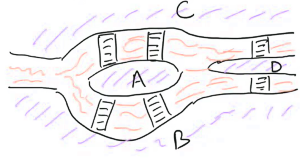
\includegraphics{reka-pregel} \\
	Problem K\"onigsber"skih mostov: ali se lahko sprehodimo tako, da gremo prek vsakega mosta natanko enkrat (in zaklju"cimo kjer smo za"celi)?
	
	\begin{definition}[Eulerjev sprehod]
		Sprehod v grafu, ki vsako povezavo prehodi natanko enkrat.
	\end{definition}
	
	\begin{definition}[Eulerjev obhod]
		Sklenjen Eulerjev sprehod.
	\end{definition}
	
	\begin{definition}[Eulerjev graf]
		Graf, ki premore Eulerjev obhod.
	\end{definition}

	\begin{claim}
		"Ce graf premore vozli"s"ce stopnje $1$, potem ni Eulerjev.
	\end{claim}

	\begin{theorem}
		Povezan graf je Eulerjev natanko tedaj, ko so vsa vozli"s"ca sode stopnje.
		\begin{proof}
			($\Rightarrow$) Naj bo $G$ Eulerjev graf. Opazujmo poljuben obhod $P$. Izberimo poljubno vozli"s"ce $x$. Povezave vozli"s"ca vedno nastopajo v parih (pot pride noter, potem gre ven). Par prve povezave je zadnja povezava. \\
			($\Leftarrow$) Naj bo $G$ poljuben povezan graf s samimi sodimi vozli"s"ci. Doka"zemo z indukcijo po $|E(G)|$.\\
			B.I. $|E(G)| = 3$ OK \\
			I.K. $|E(G)| \geq 4$. Trdimo, da G premore cikel (ker vemo, da ni drevo - ker nima listov (ki bi bili lihe stopnje)). Naj bo $C$ poljuben cikel grafa $G$. $H$ naj bo graf enak $G$ju, brez povezav cikla $C$. V grafu $H$ so spet vsa vozli"s"ca sode stopnje. $H$ v splo"snem ni povezan, toda vsaka komponenta (komponente so po definiciji povezane) ima vsa vozli"s"ca sode stopnje. Po IP vsak izmed $H_1, ... H_k$ premore Eulerjev obhod. Sedaj konstruiramo Eulerjev obhod v $G$: gibljemo se vzdol"z $C$. Br"z ko naletimo na neprehojeno komponento $H_i$, jo prehodimo.
		\end{proof}
	\end{theorem}
	\begin{claim}
		Zgornji izrek velja tudi za multigrafe. Dokaz je podoben.
	\end{claim}
	
	\begin{claim}
		Eulerjev sprehod premorejo natanko tisti grafi, ki imajo kve"cjemu 2 vozli"s"ci. "Ce jih ima 0, je to Eulerjev graf, "ce pa ima 2, ima Eulerjev sprehod. (1 lihega vozli"s"ca ne more imeti zaradi leme o rokovanju)
	\end{claim}

	\begin{theorem}[Fleuryjev algoritem]
		Za iskanje Eulerjevih obhodov. \\
		Vhod: povezan graf s samimi sodimi vozli"s"ci. \\
		Izhod: Eulerjev obhod.
		\begin{enumerate}
			\item Za"cnemo v poljuben vozli"s"cu.
			\item Gremo po poljubni povezavi, ki jo zbri"semo za seboj.
			\item Postopek ponavljamo in pri tem pazimo le na to, da naslednja izbrana povezava ni most, razen "ce ni druge mo"znosti.
			% algoritem, da ugotovimo, ce je povezava most, je standardni BFS
		\end{enumerate}
	\end{theorem}

	\begin{definition}[Dekompozicija grafa]
		Seznam podgrafov, da se vsaka povezava pojavi v natanko enem podgrafu.
	\end{definition}

	\begin{claim}
		"Ce je $G$ graf, ki ima samao soda vozli"s"ca, potem $G$ premore dekompozicijo v cikle.	
		\begin{proof}
			Vemo, da $G$ premore cikel; odstranimo ga in argument zaklju"cimo z indukcijo.
		\end{proof}
	\end{claim}

	\subsection{Hamiltonovi grafi}
	\begin{definition}[Hamiltonova pot]
		Pot, ki gre skozi vsa vozli"s"ca grafa ($V(P) = V(G)$).
	\end{definition}

	\begin{definition}[Hamiltonov cikel]
		Cikel, ki gre skozi vsa vozli"s"ca grafa ($V(C) = V(G)$).
	\end{definition}
	
	\begin{definition}[Hamiltonov graf]
		Graf, ki premore Hamiltonov cikel.
	\end{definition}

	Hamiltonova pot je vpeta pot (oz. vpet podgraf, ki je pot).
	
	Hamiltonov cikel je torej vsak vpet cikel grafa.
	
	Ali je graf Eulerjev? Ali je graf Hamiltonov?
	\begin{claim}
		''Ali je graf Hamiltonov'' je NP-poln problem. % sad
	\end{claim}

	\begin{theorem}
		"Ce je $G$ Hamiltonov graf in je $S \subseteq V(G)$, potem je
		$$\Omega(G-S) \leq |S|$$
		\begin{proof}
			Naj bo $V(G) = \left\lbrace v_1, v_2, \ldots, v_n \right\rbrace $. Ker je $G$ Hamiltonov, lahko brez "skode za splo"snost privzamemo, da je $v_1 \rightarrow v_2 \rightarrow ... \rightarrow v_n \rightarrow v_1 $ Hamiltonov cikel. 
			
			$S = \left\lbrace v_{i_1}, v_{i_2}, \ldots, v_{i_k} \right\rbrace $ \\
			$ i_1 < i_2 < \ldots < i_k $ \\
			$|S| = k$ \\
			Tedaj vozli"s"ca med $v_{i_j}$ in $v_{i_{j+1}}$ le"zijo v isti komponenti $G-S$.
			V vsakem primeru je komponent v $G-S$ kve"cjemu $k=|S|$
		\end{proof}
	\end{theorem}

	V praksi zadnji izrek uporabljamo, da dokazujemo, da graf NI Hamiltonov. Kontrapozicija izreka se namre"c glasi: 
	$$ \text{"Ce } \exists S \leq V(G): \Omega(G-S) > |S| \Rightarrow G \text{ ni Hamiltonov.}$$
	
	\begin{claim}
		"Ce ima (povezan) graf prerezno vozli"s"ce, potem ni Hamiltonov.
	\end{claim}
	\begin{claim}
		$ K_{m,n} $ je Hamiltonov $ \iff m=n $
		\begin{proof}
			($\Rightarrow$) Naj bo $m \neq n$ in B"SS $m < n$. Postavimo $S=A$. Tedaj ima graf $K_{m,n}-S$ natanko $n$ komponent (n izoliranih vosli"s"c). \\
			($\Leftarrow$)  Opazujmo $K_{m,n}$. Brez te"zav najdemo Hamiltonov cikel.
		\end{proof}
	\end{claim}

	\begin{theorem}[Orejev] % naglas na ozki O
		Naj bo $G$ graf z $|V(G)| \geq 3$. "Ce za vsak par nesosednjih vozli"s"c $u$, $v$ velja
		$$ deg(u) + deg(v) \geq |V(G)| $$
		potem je $G$ Hamiltonov.
		\begin{proof}(Z metodo najmanj"sega protiprimera)
			Recimo, da izrek ne velja. Potem obstajajo grafi, za katere velja dani pogoj, a niso Hamiltonovi. Med vsemi takimi primeri poi"s"cemo tiste, ki imajo najmanj vozli"s"c. Med vsemi takimi izberimo tistega (imenujmo $G$), ki ima najve"c povezav.
			% Situacija:
			% * G zadosca pogoju
			% * G ni hamiltonov
			% * G ima najvec povezav med vsemi protiprimeri na najmanj vozliscih
			G ni poln graf (ker poln graf je gotovo Hamiltonov), zato obstajata nesosednja $u$ in $v$. Poglejmo $G + uv$. % grafu G dodamo povezavo uv
			Ta je gotovo Hamiltonov (ker ima $G$ najve"c povezav mo"zno). Torej $G+uv$ ima Hamiltonov cikel. Ta cikel gotovo vsebuje povezavo $uv$. % logicno
			
			Definirajmo
			$$ S = \left\lbrace i; u \sim u_{i+1} \right\rbrace $$
			% S = indeksi predhodnikov sosedov u-ja
			$$ T = \left\lbrace i; u \sim u_i \right\rbrace $$
			% T = indeksi sosedov v-ja
			$$ |S \cup T| = |S| + |T| - |S \cap T| $$
			$$ |S \cup T| + |S \cap T| = |S| + |T| $$
			$$ |S| + |T| = deg(u) + deg(v) \geq_{\text{(po izreku)}} |V(G)| $$
			$$ n \not\in S \land n \not\in T $$
			$$ \Rightarrow |S \cup T| < n $$
			$$ \Rightarrow |S \cap T| \geq 1 $$
			Naj bo $i \in S \cap T$. Protislovje je o"citno.\\
			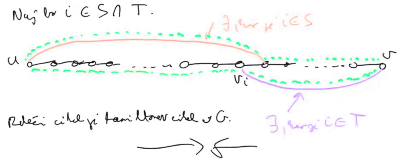
\includegraphics{orejev-izrek} \\
		\end{proof}
	\end{theorem}

	\begin{conseq}[Dirac] % pronounced "dirAkov"
		Naj bo $G$ graf z $|V(G)| \geq 3$. "Ce za vsako vozli"s"ce velja
		$$ deg(u) \geq \frac{|V(G)|}{2} $$
		potem je $G$ Hamiltonov.
		\begin{proof}
			Diracov pogoj zagotavlja, da je izpoljnjen Orejev pogoj prej"snjega izreka. Naj bosta $u$ in $v$ nesosednji vozli"s"ci v $G$. Potem je $deg(u) + deg(v) \geq \frac{|V(G)|}{2} + \frac{|V(G)|}{2} = |V(G)|$
		\end{proof}
	\end{conseq}


	% 30. 03. 2021
	\section{Ravninski grafi}
	\begin{definition}[Ravninska risba]
		Risba grafa, kjer se nobeni dve povezavi ne sekata.
	\end{definition}
	\begin{definition}[Ravninski graf]
		Graf, ki ima ravninsko risbo.
	\end{definition}

	\begin{itemize}
		\item Vsi cikli so ravninski
		\item Vsa drevesa so ravninska
		\item $K_{2,3}$ je ravninski
		\item $K_{3,3}$ ni ravninski
	\end{itemize}
		
	\begin{definition}[Graf vlo"zen v ravnini]
		"Ce imamo ravninski graf in njegovo sliko v ravnini.
	\end{definition}
	
	\begin{definition}[Enostavna krivulja]
		Krivulja, ki ne seka same sebe.
	\end{definition}
	\begin{theorem}[Jordanov]
		Enostavna sklenjena krivulja razdeli ravnino na notranjost in zunanjost.
		\begin{proof}
			Je dale"c od tega da bi bil enostaven, zato se skriva pri predmetu Topologija.
		\end{proof}
	\end{theorem}
	
	\begin{definition}[Lice]
		"Ce v ravninski risbi zbri"semo vse to"cke, ki predstavljajo povezave in vozli"s"ca, dobimo nekaj lo"cenih obmo"cij, ki jim pravimo lica vlo"zitve (ang. faces). Mno"zico vseh lic ozna"cimo $F(G)$
	\end{definition}
	
	\begin{claim}
		Graf lahko vlo"zimo v ravnino natanko tedaj, ko ga lahko vlo"zimo na sfero.
	\end{claim}
	Ker je na sferi vsako lice omejeno, lahko sklepamo, da zunanje lice ravninske risbe ''ni ni"c posebnega''.
	
	\begin{definition}[Dol"zina lica]
		"Stevilo povezav, ki jih prehodimo, ko obhodimo lice. Oznaka $l(f)$.
	\end{definition}

	\begin{claim}
		Naj bo G ravninski graf, vlo"zen v ravnino. Tedaj velja:
		$$ \sum_{f \in F(G)}l(f) = 2*|E(G)| $$
	\end{claim}
	\begin{definition}[O"zina grafa]
		Je dol"zina najkraj"sega cikla v grafu. Oznaka $g(G)$. "Ce $G$ nima cikla (je gozd), postavimo $g(G) = \infty$.
	\end{definition}

	\begin{claim}
		"Ce je $G$ povezan ravninski graf vlo"zen v ravnino, potem je
		$$ |E(G)| \geq \frac{g(G)}{2}|F(G)| $$
		\begin{proof}
			"Ce je $G$ povezan graf vlo"zen v ravnino in $f$ lice vlo"zitve, potem je $f(g) \geq g(G)$. Po prej"snji trditvi dobimo:
			$$ 2|E(G)| = \sum_{f \in F(G)}l(f) \geq \sum_{f \in F(G)} g(G) =|F(G)|*g(G) $$
		\end{proof}
	\end{claim}
	Povezanost je pomembna lastnost v prej"snjem dokazu.
	
	\begin{theorem}[Eulerjeva formula]
		Naj bo $G$ ravninski graf z vsaj eno povezavo vlo"zen v ravnino. Tedaj velja, da je
		$$|V(G)| - |E(G)| + |F(G)| = 1 + |\Omega(G)| $$
		% omega je stevilo komponent G
		
		% euler je poenostavljeno formulo (za omega(G) = 2) dokazal s poliedri
		% what a chad
		
		% OP: poliedri so basically 3-povezani ravninski grafi
		
		\begin{proof}Z indukcijo po $|E(G)|$. \\
			BI. $|E(G)| = 1 \Rightarrow 2 - 1 + 1 = 1 + 1$ OK \\
			Formula velja za vsa drevesa.
			$$ |V(T)| - |E(T)| + |F(T)| = |V(T)| - (|V(T)|-1) + 1 = 2 $$
			Sicer naj bo $G$ poljuben povezan ravninski graf z $n \geq 3$ vlo"zen v ravnino z vsaj enim ciklom $C$. \\
			IK. Vzemimo povezavo $e$ iz $C$. Vemo, da je $G-e$ povezan. Je tudi ravninski graf, in je vlo"zen v ravnino. Ker je $|E(G-e)| = n-1$, po IP velja Eulerjeva formula.
			$$|V(G-e)| - |E(G-e)| + |F(G-e)| = 2 $$
			$$|V(G)| - (|E(G)|-1) + (|F(G)|-1) = 2 $$
			$-1$ se od"steje ...
			$$|V(G)| - |E(G)| + |F(G)| = 2 $$
			
			"Ce graf ni povezan, uporabimo Eulerjevo formulo za vsako komponento posebej in zdru"zimo rezultat.
		\end{proof}
	\end{theorem}

	\begin{conseq}[Sporo"cilo Eulerjeve formule]
		Ne glede na to, kako nari"semo graf v ravnini, ima enako "stevilo lic.
		$$ |F(G)| = - |V(G)| + |E(G)| + 2 $$
	\end{conseq}
	
	\begin{conseq}
		"Ce je $G$ povezan ravninski graf, ki ni drevo, potem je
		$$ |E(G)| \leq \frac{g(G)}{g(G)-2}(|V(G)|-2) $$
		\begin{proof}
			Trditev od prej:
			$$ |E(G)| \geq \frac{g(G)}{2}|F(G)| $$
			$$ |F(G)| \leq \frac{2*|E(G)|}{g(G)} $$
			Po Eulerjevi formuli dobimo:
			$$ 2 = |V(G)| - |E(G)| + |F(G)| \leq $$
			$$ \leq |V(G)| - |E(G)| + \frac{2|E(G)|}{g(G)} = $$
			$$ = |V(G)| - |E(G)|(\frac{g(G)-2}{g(G)}) $$
			
			$$ |E(G)|(\frac{g(G)-2}{g(G)}) \leq |V(G)| -2 \Rightarrow $$
			$$ |E(G)| \leq \frac{g(G)}{g(G)-2}(|V(G)|-2) $$
		\end{proof}
	\end{conseq}
	
	Ker je $g(G) \geq 3$ in $\frac{g(G)}{g(G)-2} \leq 3$, za VSAK ravninski graf, velja
	$$ |E(G)| \leq 3|V(G)|-6 $$
	"Ce ima cikel, to sledi iz zadnje posledice, "ce pa je drevo, pa itak vemo, da je $|E(G)| = |V(G)| - 1$.
	
	"Ce pa je $G$ ravninski graf brez trikotnikov in z vsaj 3 vozli"s"ci, potem velja:
	$$ |E(G)| \leq 2|V(G)| - 4 $$
	
	Ti dve formuli sta pomembni tudi zato, ker nam data linearno oceno za "stevilo povezav ravninskega grafa.
	
	
	Kako ugotovimo ali je graf ravninski?
	\begin{itemize}
		\item "Ce je, potem doka"zemo tako, da podamo vlo"zitev v ravnino
		\item "Ce ni, potem uporabimo izrek Karatowskega ali Wagnerjev izrek
	\end{itemize}
	\begin{theorem}[Karatowski]
		Graf je ravninski natanko tedaj, ko ne vsebuje podgrafa izomorfnega subdiviziji grafa $K_5$ ali subdiviziji $K_{3,3}$.
		\begin{proof}
			V eno smer je skoraj o"citno.
			\begin{itemize}
				\item $K_{3,3}$ in $K_5$ nista ravninska
				\item $G$ je ravninski $\iff$ vsaka njegova subdivizija je ravninska.
			\end{itemize}
			V drugo smer, je predolg % in potem se par minut flexa o tem kako so ''kratki dokazi'' dolgi 2-3h
		\end{proof}
	\end{theorem}
	\begin{theorem}[Wagner]
		Graf je ravninski natanko tedaj, ko nima minorja izmorfnega s $K_5$ ali $K_{3,3}$
		% minor dobimo tako, da iz nekega podgrafa skrcimo nekaj povezav
	\end{theorem}

	% 06. 04. 2021
	\section{Barvanje grafov}
	\begin{definition}[Barvanje grafa]
		Je preslikava, ki vsakemu vozli"s"cu v grafu priredi barvo.
	\end{definition}
	\begin{definition}[Dobro barvanje]
		Sosednji vozli"s"ci se preslikata v razli"cni barvi.
		$$ \forall u,v \in E(G): c(u) \neq c(v) $$
	\end{definition}
	\begin{definition}[(dobro) $k$-barvanje]
		(Dobro) barvanje, kjer za mno"zico barv $K$ velja $|K| = k$
	\end{definition}
	\begin{definition}[Kromati"cno "stevilo]
		Najmanj"si $k$, za katerega obstaja $k$-barvanje grafa. Ozna"cimo z $\chi(G)$
	\end{definition}
	Od tu dalje barvanje pomeni dobro barvanje.
	
	$\chi(K_n) = n$ \\ $\chi(C_n) = 2\text{, "ce je }n\text{ sod, sicer }3$ \\ $\chi(P) = 3$
	
	\begin{definition}[Barvni razredi]
		Mno"zice vozli"s"c iste barve.
	\end{definition}
	Bistvo je, da znotraj barvnega razreda ni povezav. Re"cemo, da so barvni razredi neodvisne mno"zice.
	
	Kako dolo"cimo $\chi(G)$?
	Poi"s"cemo $k$, da velja:
	\begin{itemize}
		\item $\chi(G) \leq k$
		\item $\chi(G) \geq k$
	\end{itemize}
	Konstrukcija: poi"s"cemo $k$-barvanje. Potrebujemo dokaz, da ne gre z manj kot $k$ barvami. Na primer, poi"s"cemo $C_k$ kot podgraf.
	\begin{claim}
		"Ce je $H$ podgraf $G$, velja $\chi(G) \geq \chi(H)$
		\begin{proof}
			Trditev o"citno velja.
		\end{proof}
	\end{claim}

	\subsection{Po"zre"sni algoritem barvanja}
	Barve si od tu dalje predstavljamo kot naravna "stevila. Natan"cneje, $k$-barvanje pomeni $c: V(G) \rightarrow [k]$
	
	Naj bo G graf z vosli"s"ci $v_1,v_2,...,v_k$. Po tem vrstnem redu barvamo vozli"s"ca tako, da uporabimo najmanj"so mo"zno barvo (najmanj"sa, ki "se ni uporabljena na nobenem od sosedov).\\
	O"citno je rezultat algoritma odvisen od ostevil"cenja vozli"s"c.
	
	\begin{claim}
		Po"zre"sni algoritem je lahko poljubno slab
		\begin{proof}
			Iz grafa $K_{n,n}$ odstranimo vse ''navpi"cne'' povezave. Po"zenemo po"zre"sni algoritem, ki vrne $\chi=n$. Vemo pa, da je $K_{n,n}$ dvodelen, torej bi morali dobiti $\chi=2$.
			\\ 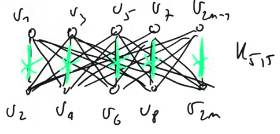
\includegraphics{navpicne} \\
		\end{proof}
	\end{claim}
	\begin{claim}
		Vedno obstaja tak vrstni red vozli"s"c, da po"zre"sni algoritem vrne pravilen rezultat.
	\end{claim}

	\begin{claim}
		"Ce je G graf, potem je $\chi(G) \leq \Delta(G) + 1$
		\begin{proof}
			Po"zenemo po"zre"sni algoritem v poljubnem vrstnem redu. Ko barvamo $v$, ima kve"cjemu $deg(v)$ pobarvanih sosedov. $$deg(v) \leq \Delta(G)$$
			Zato v mno"zici barv $[\Delta(G)+1]$ obstaja barva, ki jo po"zre"sni algoritem lahko uporabi za barvo vozli"s"ca $v$. Torej smo vsa vozli"s"ca pobarvali z eno izmed barv iz $[\Delta(G)+1]$.
		\end{proof}
	\end{claim}

	\begin{claim}
		"Ce $G$ ni regularen graf, potem je $\chi(G) \leq \Delta(G)$.
		\begin{proof}
			Naj bo $v$ vozli"s"ce, za katerega velja $deg(v) < \Delta(G)$ (obstaja, ker graf ni regularen). Opazujmo BFS drevo iz $v$. Sedaj po"zenemo po"zre"sni algoritem v vrstnem redu $n, n-1, n-2, ..., 1$. Ko barvamo poljubno vozli"s"ce $x \neq v$, ima $x$ vsaj enega nepobarvanega soseda: torej je v mno"zici $[\Delta(G)]$ vsaj ena prosta barva. Ta zaklju"cek pa velja tudi za barvanje zadnjega vozli"s"ca $v$, saj je $deg(v) < \Delta(G)$.
		\end{proof}
	\end{claim}
	Opomba: pogoj regularnosti v zadnji trditvi potrebujemo.
	
	\begin{theorem}[Brooks]
		"Ce je $G$ povezan graf, ki ni cikel lihe dol"zine in ni polni graf, potem velja 
		$$\chi(G) \leq \Delta(G)$$
		\begin{proof}
			Nima preprostega dokaza. Morda na drugi stopnji.
		\end{proof}
	\end{theorem}
	
	Slavni problem 4 barv: ali lahko vedno pobarvamo zemljevid tako, da vsaki sosednji dr"zavi prejmeta razli"cni barvi in za to porabimo kve"cjemu 4 barve?
	% predpostavljamo, da za sosednjost potrebujemo ve"c kot 1 skupno to"cko
	
	% Storytime:
	% nekdo je enrat naredu dokaz, ampak so kasnej najdl napako
	% cez 100 let je nekdo drug naredu racunalniski dokaz (100 strani + lots of cpu time required)
	% mal kasnej se nekdo skrajsa dokaz amapak se zmeri ni kombinatoricen, ampak rabs cpu
	% kombinatoren dokaz za ta problem obstaja odprto vprasanje.
	
	\begin{theorem}[4 barv]
		"Ce je $G$ ravninski graf, potem je $\chi(G) \leq 4$.
	\end{theorem}
	
	\subsection{Barvanje povezav}
	\begin{definition}[$k$-barvanje povezav]
		je preslikava $c: E(G) \rightarrow [k]$. "Ce gre za dobro barvanje, velja:
		$$ \forall uv, uw \in E(G) \Rightarrow c(uv) \neq c(uw) $$
	\end{definition}
	\begin{definition}[Kromati"cni indeks]
		Najmanj"si $k$, za katerega obstaja barvanje povezav $G$. Ozna"cimo $\chi'(G)$.
		% notacija, kjer crtica pomeni analogni koncept v povezavah (namesto vozli"s"cih) je ''precej standardiziran''
	\end{definition}

	\begin{claim}
		$\chi'(G) \geq \Delta(G)$
	\end{claim}

	\begin{theorem}[Vizing]
		Za vsak graf $G$ velja $$ \Delta(G) \leq \chi'(G) \leq \Delta(G)+1 $$
		\begin{proof}
			"Ce imate dokaz ki se po nekom imenuje, potem je verjetno izven obsega na"sega predmeta.
		\end{proof}
	\end{theorem}
	Torej: $\chi'(G) \in \lbrace \Delta(G), \Delta(G)+1 \rbrace$
	
	\begin{definition}[Razred grafa]
		Graf $G$ je razreda 1, "ce je $\chi'(G) = \Delta(G)$. V nasprotnem primeru mora veljati $\chi'(G) = \Delta(G)+1$, $G$ pa je razreda 2.
	\end{definition}

	\begin{theorem}
		"Ce je $n$ sod, je $K_n$ razreda 1, sicer je razreda 2.
		\begin{proof}
			Naj bo najprej $n=2k+1$. Pobarvajmo povezave takole: zamislimo si pravilen $(2k+1)$-kotnik in povezave vzdol"z tega poligona pobarvajmo z barvami $1,2,...,2k+1$. Vsaka nadaljna povezava je vzpredna z eno stranico $(2k+1)$-kotnika. Sedaj te preostale povezave (tetive) pobarvamo z isto barvo, kot jo ima vzporedna povezava $(2k+1)$-kotnika. Ker vzporedne povezave nimajo skupnih kraji"s"c, je to dobro barvanje povezav $K_{2k+1}$ z $2k+1$ barvami.
			$$ \Rightarrow \chi'(K_{2k+1}) \leq 2k+1 = \Delta(G)+1 $$
			
			Doka"zimo "se, da $\chi'(K_{2k+1}) \geq 2k+1$.
			Recimo nasprotno: $K_{2k+1}$ smo uspeli po povezavah pobarvati s samo $2k$ barvami.
			Koliko najve"c povezav lahko pobarvamo z isto barvo? Kve"cjemu $k$, ker vsaka povezava ''zasede'' dve kraji"s"ci zase.
			Ker imamo $2k$ barv, smo torej pobarvali $\leq (2k)*k$ povezav.
			Na"se barvanje je pobarvalo kve"cjemu $2k^2$ povezav. Vemo pa, da je $$ |E(K_{2k+1})| = \binom{2k+1}{2} = \frac{(2k+1)*2k}{2} = 2k^2 + k$$
			Torej imamo ve"c barv kot smo jih lahko pobarvali, kar je protislovje.
			$$ \Rightarrow \chi'(K_{2k+1}) \geq 2k+1$$
			$$ \Rightarrow \chi'(K_{2k+1}) = 2k+1\text{, torej je razreda 2}$$
			
			Naj bo sedaj $n=2k$. Lahko ga dobimo iz $K_{2k-1}$ tako, da dodamo novo vozli"s"ce, ki ga pove"zemo z vsemi vozli"s"ci iz $K_{2k-1}$.
			Sedaj povezave v $K_{2k-1}$ pobarvamo z zgoraj opisano konstrukcijo.
			Vsakemu vozli"s"cu tedaj ''manjka'' ena barva; tista, s katero smo pobarvali temu vozli"s"cu nasprotno stranico. S to barvo pobarvamo povezavo do novo dodalega vozli"s"ca.
			\\ 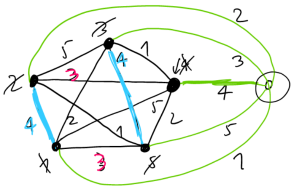
\includegraphics{barvanje-kn} \\
			S tem smo dodali vse prej obstoje"ce barve in dobili barvanje za $K_{2k}$. Torej smo porabili
			$$ \Delta(K_{2k-1})+1 = \Delta(K_{2k}) $$
			barv. Ker velja tudi
			$$ \chi'(K_{2k}) \geq \Delta(K_{2k})$$
			$$\implies \chi'(K_{2k}) = \Delta(K_{2k}) $$
			torej je $K_{2k}$ razreda 1.
			% no, pa smo ugnali polne grafe
		\end{proof}
	\end{theorem}

	\begin{theorem}
		"Ce je $G$ dvodelen graf, potem je $G$ razreda 1.
		\begin{proof} Z indukcijo po $|E(G)|$ \\
			B"SS naj bo $G$ povezan.\\
			BI: $\Delta(K_2) = 1 = \chi'(K_2)$ OK \\
			$G$ je poljuben povezan dvodelen graf in $uv = e \in E(G)$. \\
			$H := G-e$. \\
			Po IP (ker je $H$ tudi dvodelen): $\chi'(H) = \Delta(H)$. "Ce je $\Delta(H) < \Delta(G)$, potem je seveda tudi $G$ razreda 1; povezavo $e$ pobarvamo s svojo barvo. 
			Naj bo torej $\Delta(H) = \Delta(G)$. Naj bo $c$ poljubno optimalno barvanje povezav grafa $H$. Opazujmo vozli"s"ce $u \in e$.
			To vozli"s"ce je v $H$ stopnje $< \Delta(H)$ (ker smo eno njegovo povezavo odstranili).
			Zato v barvanju $c$ pri vozli"s"cu $u$ manjka vsaj ena barva iz mno"zice $[\Delta(H)]$. Naj bo to barva $\alpha$.
			Analogno sklepamo, da pri $v \in e$ manjka ena barva iz $[\Delta(H)]$, naj bo to $\beta$.
			\begin{itemize}
				\item "Ce je $\alpha = \beta$:\\
				Povezavo $uv$ lahko tedaj pobarvamo z $\alpha$ in zaklju"cimo indukcijski korak.
				
				\item "Ce $\alpha \neq \beta$:\\
				Vemo, da iz $u$ poteka povezava barve $\beta$ (sicer bi to lahko obravnavali kot zgornji primer $\alpha = \beta$).
				
				Naredimo cik-cak pot $P$ (ki se za"cne v $u$), ki sledi izmeni"cno najprej barvi $\alpha$, nato $\beta$. V neki to"cki bomo naleteli na vozli"s"ce, ki nima povezave z ustrezno barvo. Tam pot zaklju"cimo.
				\\ 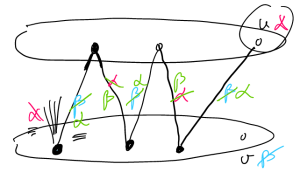
\includegraphics{cik-cak-dvodelni} \\
				Potem na tej poti zamenjamo $\alpha$ in $\beta$. Novo barvanje je "se vedno dobro barvanje, toda sedaj v vozli"s"cu $u$ manjka $\beta$ namesto $\alpha$. Ker tudi v $v$ manjka $\beta$, lahko $e$ pobarvamo z $\beta$. To zaklju"ci IK.
				% zaklju"ci tudi ta dokaz, in trenutno poglavje, in tudi zakljuci celotno teorijo grafov.
			\end{itemize}
		\end{proof}
	\end{theorem}

	% end of graph theory
\end{document}






